\section{MCMC采样}
\label{sec:sgen-mcmc}

直接生成要求一次性造出一个完整的目标样本，这需要分位数、可抽样的分解或贴身的包络。高维目标往往三者都没有，能做的只是逐点计算未归一化密度$\widetilde{p}(x)$，或者计算它的梯度。只靠这些局部信息，能否得到目标分布的样本？

\term{Markov链Monte Carlo}（Markov chain Monte Carlo，MCMC）的回答是：不再从头造样本，而是让一个状态在空间中游走，每一步只根据当前位置随机地走到下一个位置，并设计走法，使目标概率大的地方被访问得更频繁。把目标分布想象成地形的高度，游走者在高处停留得久、在低处停留得短，长时间下来，在各处停留的时间比例就接近目标概率。这个图景有两处需要准确化：“走法不破坏目标分布”是一个可以逐步验证的代数条件，即下面的不变性；“长时间后停留比例接近目标”则还需要链能走遍目标的支持，这是另一个条件，不能由第一个推出。

本节先建立转移与不变分布，再介绍保持目标不变的三种更新，它们分别以Metropolis--Hastings、Gibbs和Hamilton命名。它们的输出都是一串相关的状态，而不是独立样本。

\subsection{转移与不变分布}
\label{sec:sgen-invariance}

\paragraph{转移核}
链式更新的每一步，都是在给定当前状态$x$时，随机地选出下一个状态。把“给定$x$时下一状态的分布”记作$K(x,\cdot)$：对状态空间中的集合$A$，$K(x,A)$是从$x$出发一步后进入$A$的概率。按第~\ref{chap:conditional-distributions}章的定义，$K$是从状态空间到自身的概率核，在这里称为\term{转移核}（transition kernel）。状态有限时，$K$就是一个每行和为$1$的非负矩阵，第$x$行第$y$列为$K(x,\{y\})$。

用转移核生成一条链：给定初始状态$X^{(0)}$，对$t=0,1,2,\dots$，用新的基础随机数从$K(X^{(t)},\cdot)$中抽出$X^{(t+1)}$。具体实现中，常写成$X^{(t+1)}=\Psi(X^{(t)},\bm{U}^{(t+1)})$，其中$\Psi$是确定的更新函数，$\bm{U}^{(t+1)}$是第$t+1$步专用的基础随机数，并且对每个$x$，$\Psi(x,\bm{U})$的分布是$K(x,\cdot)$。由于各步的随机数互不重叠，给定$X^{(t)}$后，$X^{(t+1)}$与更早的状态无关，这正是Markov链的含义，第~\ref{chap:information-measures}章对三个变量用过的Markov性在这里对整个序列成立。

\paragraph{分布的传播}
若$X^{(t)}$的分布是$\mu_t$，下一步的分布是多少？$\bm{U}^{(t+1)}$与$X^{(t)}$独立，给定$X^{(t)}=x$时$X^{(t+1)}$的条件分布是$K(x,\cdot)$。由第~\ref{chap:conditional-distributions}章边缘分布与概率核复合的公式，
\begin{equation}
  \mu_{t+1}(A)=\int K(x,A)\,\mu_t(\mathrm{d}x),\qquad\text{记作}\quad\mu_{t+1}=\mu_tK .
  \label{eq:sgen-distribution-step}
\end{equation}
状态有限时，这就是行向量乘矩阵：$\mu_{t+1}=\mu_t\bm{K}$。

\paragraph{不变分布}
如果某个分布在一步更新后不变，从它出发就永远保持在它上面。

\begin{definition}[不变分布]
\label{def:sgen-invariant}
若状态空间上的概率分布$\pi$对一切可测集$A$满足
\begin{equation}
  \int K(x,A)\,\pi(\mathrm{d}x)=\pi(A),
  \label{eq:sgen-invariance}
\end{equation}
即$\pi K=\pi$，则称$\pi$是转移核$K$的\term{不变分布}（invariant distribution），也称平稳分布。
\end{definition}

若$X^{(0)}\sim\pi$且$\pi$是不变分布，由式~\eqref{eq:sgen-distribution-step}按$t$归纳，每个$X^{(t)}$的边缘分布都是$\pi$。这时链的每一个状态单独看都是目标分布的样本，只是相邻状态之间一般不独立。MCMC构造的第一个要求，就是让目标分布$\pi$成为转移核的不变分布。

用一个三状态的例子检验定义。取状态$\{1,2,3\}$上的转移矩阵
\[
  \bm{K}=\begin{bmatrix}0.5&0.5&0\\0.2&0.5&0.3\\0&0.5&0.5\end{bmatrix},\qquad \pi=(0.2,0.5,0.3).
\]
逐列计算$\pi\bm{K}$：
\[
  \begin{aligned}
    (\pi\bm{K})_1&=0.2\times0.5+0.5\times0.2=0.2,\\
    (\pi\bm{K})_2&=0.2\times0.5+0.5\times0.5+0.3\times0.5=0.5,\\
    (\pi\bm{K})_3&=0.5\times0.3+0.3\times0.5=0.3,
  \end{aligned}
\]
所以$\pi$是不变分布。若从状态$1$出发，$\mu_0=(1,0,0)$，按式~\eqref{eq:sgen-distribution-step}逐步计算，
\[
  \mu_1=(0.5,0.5,0),\qquad \mu_2=(0.35,0.5,0.15),\qquad \mu_3=(0.275,0.5,0.225),
\]
各分量一步步向$\pi$靠拢。图~\ref{fig:sgen-chain-evolution}(a)画出了前几步，(b)是沿一条模拟路径计算的“停在状态$3$的时间比例”，它在约$2000$步后接近$0.3$。

\begin{BookInlineFigure}
  \centering
  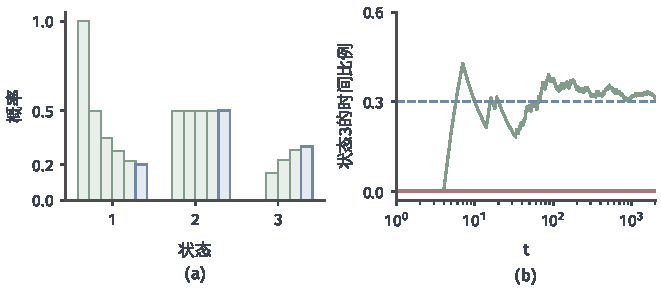
\includegraphics[width=112mm]{figures/07-probability/08-sampling-and-integration/matplotlib/sgen-chain-evolution/figure.pdf}
  \caption{三状态转移矩阵$\bm{K}$的分布传播与时间平均。(a)从状态$1$出发，每组左起五根绿色柱依次是$t=0,1,2,3,5$时的$\mu_t$，最右的蓝色柱是不变分布$\pi=(0.2,0.5,0.3)$；(b)一条模拟路径（种子$6$，横轴为对数刻度）上停在状态$3$的时间比例，绿线是$\bm{K}$，红线是“永远停在原地”的转移，蓝色虚线是$\pi(\{3\})=0.3$。}
  \label{fig:sgen-chain-evolution}
\end{BookInlineFigure}

\paragraph{不变不等于能到达}
不变性只说“从目标出发会留在目标”，不说“从别处出发会走到目标”。最极端的例子是始终停在原地的转移$K(x,\cdot)=\delta_x$，即单位矩阵。对它而言，任何分布都满足式~\eqref{eq:sgen-invariance}，目标分布当然也是不变分布。但从状态$1$出发，链永远停在$1$，停在状态$3$的时间比例恒为$0$，与$\pi(\{3\})=0.3$毫无关系，这就是图~\ref{fig:sgen-chain-evolution}(b)中的红线。

不那么极端的失败也很常见。若转移矩阵是分块对角的，例如状态$\{1,2\}$与$\{3\}$之间互不往来，从块$\{1,2\}$出发就永远看不到状态$3$。若转移在两个状态之间交替，$\bm{K}=\begin{bmatrix}0&1\\1&0\end{bmatrix}$，那么$(1/2,1/2)$是不变分布，从状态$1$出发的分布却在$(1,0)$与$(0,1)$之间来回摆动，永远不收敛，尽管时间比例趋于$1/2$。

所以MCMC的正确性分成两层。第一层是不变性，它是转移核的一个代数性质，下面三种更新都给出完整证明。第二层是从任意初值出发，分布收敛到$\pi$、时间平均收敛到目标期望，这需要状态之间能够互相到达（不可约）、链不陷入周期摆动（非周期）等条件。有限状态时，在不可约与非周期之下这两个结论都成立；一般状态空间需要更细的条件。这些长期性质的条件与证明可参考\BookChapterRef{chap:discrete-time-stochastic-processes}{卷九第3章“离散时间随机过程”}，也可查阅~\scite{math-meyn2009markov}。本章只证明不变性，并对每种更新指出它可能在哪里不能走遍目标。

\subsection{Metropolis--Hastings采样}
\label{sec:sgen-mh}

怎样构造一个以给定$\pi=\widetilde{p}/Z$为不变分布的转移？手里通常有一个容易抽样的局部建议，例如“在当前点附近随机迈一步”。这个建议本身一般不保持$\pi$，Metropolis--Hastings的做法是在建议之后加一道接受判定，把它修正成保持$\pi$的转移\scite{pgm-history-metropolis1953}\scite{pgm-history-hastings1970}。

\paragraph{主要思想：平衡每一对方向的概率流}
把$\pi$想象成状态之间的质量分配，转移一步就是把每个状态上的质量按转移概率分给各个状态。从$x$流向$y$的质量是$\pi(x)K(x,y)$，称为概率流。若每一对状态之间两个方向的流量相等，
\begin{equation}
  \pi(x)K(x,y)=\pi(y)K(y,x),
  \label{eq:sgen-detailed-balance-discrete}
\end{equation}
那么每个状态流出多少就流入多少，分布保持不变。这个条件称为\term{细致平衡}（detailed balance）。一般状态空间上，细致平衡写成对一切可测集$A,B$，
\begin{equation}
  \int_{A}K(x,B)\,\pi(\mathrm{d}x)=\int_{B}K(y,A)\,\pi(\mathrm{d}y),
  \label{eq:sgen-detailed-balance}
\end{equation}
即“从$A$流进$B$”等于“从$B$流进$A$”。

\begin{lemma}[细致平衡蕴含不变性]
\label{lem:sgen-detailed-balance}
若$\pi$与$K$满足式~\eqref{eq:sgen-detailed-balance}，则$\pi$是$K$的不变分布。
\end{lemma}

\begin{proof}
在式~\eqref{eq:sgen-detailed-balance}中取$A$为整个状态空间。左边是$\int K(x,B)\,\pi(\mathrm{d}x)$；右边中$K(y,\cdot)$是概率分布，$K(y,A)=1$，所以右边等于$\pi(B)$。这正是式~\eqref{eq:sgen-invariance}。
\end{proof}

细致平衡是充分条件而不是必要条件：沿圆周单向转圈的转移保持均匀分布不变，却在每一对方向上只有单向流量。它的好处是只需逐对检查，不必求和或积分，所以是构造转移最方便的工具。

现在设建议在状态$x$处的密度为$q(y\mid x)$（离散时是概率，连续时是关于Lebesgue测度的密度）。只用建议时，从$x$到$y$的流量正比于$\widetilde{p}(x)q(y\mid x)$，反向流量正比于$\widetilde{p}(y)q(x\mid y)$，二者一般不等。办法是把较大的一边按比例削减到较小的一边：从$x$到$y$的建议以概率$a(x,y)$接受，使
\[
  \widetilde{p}(x)q(y\mid x)a(x,y)=\min\bigl\{\widetilde{p}(x)q(y\mid x),\ \widetilde{p}(y)q(x\mid y)\bigr\}.
\]
右边关于$x,y$对称，流量自然平衡。解出$a$，得到
\begin{equation}
  a(x,y)=\min\Bigl\{1,\ \frac{\widetilde{p}(y)\,q(x\mid y)}{\widetilde{p}(x)\,q(y\mid x)}\Bigr\}.
  \label{eq:sgen-mh-acceptance}
\end{equation}
较小的一边接受概率为$1$，较大的一边按比值削减；被拒绝时留在原地。比值中$\widetilde{p}$出现在分子和分母，归一化常数$Z$约掉了，算法从头到尾不需要$Z$。

比值的定义需要交代。设当前状态$x$满足$\widetilde{p}(x)>0$，候选$y$由$q(\cdot\mid x)$产生，于是$q(y\mid x)>0$（概率为一），分母为正。若$\widetilde{p}(y)=0$或$q(x\mid y)=0$，比值为$0$，候选必被拒绝，所以链从$\{\widetilde{p}>0\}$出发就永远留在其中。

\begin{definition}[Metropolis--Hastings转移]
\label{def:sgen-mh}
设$\widetilde{p}\ge0$，$0<Z<\infty$，$S=\{x:\widetilde{p}(x)>0\}$。对$x\in S$，从$q(\cdot\mid x)$抽候选$y$，以式~\eqref{eq:sgen-mh-acceptance}的概率$a(x,y)$接受（令$X^{(t+1)}=y$），否则令$X^{(t+1)}=x$。对应的转移核为
\begin{equation}
  K(x,B)=\int_{B}q(y\mid x)\,a(x,y)\,\lambda(\mathrm{d}y)+r(x)\,\mathbf{1}_{B}(x),
  \label{eq:sgen-mh-kernel}
\end{equation}
其中$\lambda$是参考测度（计数测度或Lebesgue测度），
\begin{equation}
  r(x)=1-\int q(y\mid x)\,a(x,y)\,\lambda(\mathrm{d}y)
  \label{eq:sgen-mh-reject}
\end{equation}
是被拒绝而留在原地的概率。这种转移称为\term{Metropolis--Hastings算法}（Metropolis--Hastings algorithm）。
\end{definition}

\begin{theorem}[Metropolis--Hastings转移保持目标]
\label{thm:sgen-mh}
在定义~\ref{def:sgen-mh}的条件下，$\pi=\widetilde{p}/Z$与$K$满足细致平衡，因而$\pi$是$K$的不变分布。
\end{theorem}

\begin{proof}
对$\lambda$下的密度$\pi(x)=\widetilde{p}(x)/Z$，令
\[
  m(x,y)=\pi(x)\,q(y\mid x)\,a(x,y).
\]
先证
\[
  m(x,y)=\frac1Z\min\bigl\{\widetilde{p}(x)q(y\mid x),\ \widetilde{p}(y)q(x\mid y)\bigr\}.
\]
若$\widetilde{p}(x)q(y\mid x)>0$，把式~\eqref{eq:sgen-mh-acceptance}代入，乘开即得。若$\widetilde{p}(x)q(y\mid x)=0$，左边为零，右边的最小值也为零。所以$m(x,y)=m(y,x)$。

对可测集$A,B$，由式~\eqref{eq:sgen-mh-kernel}，
\[
  \int_{A}K(x,B)\,\pi(\mathrm{d}x)=\int_{A}\int_{B}m(x,y)\,\lambda(\mathrm{d}y)\,\lambda(\mathrm{d}x)+\int_{A\cap B}r(x)\,\pi(\mathrm{d}x).
\]
被积函数非负，可以交换积分次序；再用$m$的对称性，第一项对$A$与$B$对称。第二项是$r\pi$在$A\cap B$上的积分，本身对$A$与$B$对称。于是式~\eqref{eq:sgen-detailed-balance}成立，由引理~\ref{lem:sgen-detailed-balance}，$\pi$是不变分布。
\end{proof}

证明只用到两件事：接受概率使双向流量对称，被拒绝的质量留在原地。建议分布可以是任何能抽样、能计算密度的分布，这是Metropolis--Hastings的灵活之处。

\paragraph{为什么需要建议比}
若建议对称，$q(y\mid x)=q(x\mid y)$，式~\eqref{eq:sgen-mh-acceptance}简化为$\min\{1,\widetilde{p}(y)/\widetilde{p}(x)\}$，称为\term{Metropolis算法}（Metropolis algorithm）。模拟退火中的接受规则$\min\{1,\exp(-(f(y)-f(x))/T)\}$就是取$\widetilde{p}=\exp(-f/T)$的Metropolis规则。建议不对称时若仍用这个简化的比值，不变分布就会偏离目标，下面的三状态例子会算出偏离的结果。$q(x\mid y)/q(y\mid x)$这一项就是对建议偏向的修正：建议更爱往$y$走，就相应减少往$y$走的接受。

\paragraph{计算过程}
用$\{1,2,3\}$上的目标$\widetilde{p}=(2,5,3)$演示，$Z=10$对算法未知，$\pi=(0.2,0.5,0.3)$。建议在一条链上移动：从$1$总是建议$2$，从$3$总是建议$2$，从$2$以各$1/2$的概率建议$1$或$3$。建议不对称，例如$q(2\mid1)=1$而$q(1\mid2)=1/2$。

\needspace{6\baselineskip}
\paragraph{变量}
\begin{itemize}
  \item $x$：当前状态；$y$：候选状态。
  \item $a$：本步的接受概率，由式~\eqref{eq:sgen-mh-acceptance}计算。
  \item $u_{\mathrm{q}}$、$u_{\mathrm{a}}$：每步的两个基础随机数，前者用于抽候选（只在状态$2$需要），后者用于接受判定。
\end{itemize}

\paragraph{初始化}
取$x^{(0)}\in S$。例中$x^{(0)}=1$。四种可能的移动对应的接受概率可以预先算好：
\[
  \begin{aligned}
    a(1,2)&=\min\Bigl\{1,\frac{5\times\frac12}{2\times1}\Bigr\}=1,&\qquad
    a(2,1)&=\min\Bigl\{1,\frac{2\times1}{5\times\frac12}\Bigr\}=0.8,\\
    a(2,3)&=\min\Bigl\{1,\frac{3\times1}{5\times\frac12}\Bigr\}=1,&\qquad
    a(3,2)&=\min\Bigl\{1,\frac{5\times\frac12}{3\times1}\Bigr\}=\frac56.
  \end{aligned}
\]

\needspace{6\baselineskip}
\paragraph{每轮更新}
在第$t+1$步：
\begin{enumerate}
  \item \textbf{抽候选。}从$q(\cdot\mid x^{(t)})$抽$y$。例中状态$2$处，$u_{\mathrm{q}}\le0.5$时建议$1$，否则建议$3$；第一步$x^{(0)}=1$，候选$y=2$。

  \item \textbf{计算接受概率。}按式~\eqref{eq:sgen-mh-acceptance}计算$a(x^{(t)},y)$。例中第一步$a(1,2)=1$。

  \item \textbf{判定。}若$u_{\mathrm{a}}\le a$，令$x^{(t+1)}=y$；否则$x^{(t+1)}=x^{(t)}$。例中第一步$u_{\mathrm{a}}=0.37\le1$，接受，$x^{(1)}=2$。

  后四步使用的随机数与结果如下（空格表示该步不需要$u_{\mathrm{q}}$）：
  \begin{center}
    \small
    \begin{tabular}{@{}ccccccc@{}}
      \toprule
      $t$ & $x^{(t-1)}$ & $u_{\mathrm{q}}$ & $y$ & $a$ & $u_{\mathrm{a}}$ & $x^{(t)}$\\
      \midrule
      $2$ & $2$ & $0.62$ & $3$ & $1$ & $0.90$ & $3$（接受）\\
      $3$ & $3$ & & $2$ & $5/6$ & $0.88$ & $3$（拒绝）\\
      $4$ & $3$ & & $2$ & $5/6$ & $0.41$ & $2$（接受）\\
      $5$ & $2$ & $0.20$ & $1$ & $0.8$ & $0.85$ & $2$（拒绝）\\
      \bottomrule
    \end{tabular}
  \end{center}

  \item \textbf{停止。}做满预定的步数后停止。链本身没有自然的终点，步数要按下一章的误差分析决定。
\end{enumerate}
最终得到状态序列$1,2,3,3,2,2$。被拒绝的两步都把当前状态重复记录了一次，这些重复是转移的一部分，必须保留：删掉它们，状态$3$与状态$2$被访问的频率就会改变。

把接受概率乘上建议概率，得到转移矩阵
\[
  \bm{K}=\begin{bmatrix}0&1&0\\0.4&0.1&0.5\\0&\frac56&\frac16\end{bmatrix},
\]
其中$K(2,2)=1-0.4-0.5=0.1$与$K(3,3)=1/6$来自拒绝。逐对验证细致平衡：
\[
  \pi(1)K(1,2)=0.2=\pi(2)K(2,1),\qquad \pi(2)K(2,3)=0.25=\pi(3)K(3,2).
\]
图~\ref{fig:sgen-mh-three-state}画出建议与修正后的转移。

\begin{BookInlineFigure}
  \centering
  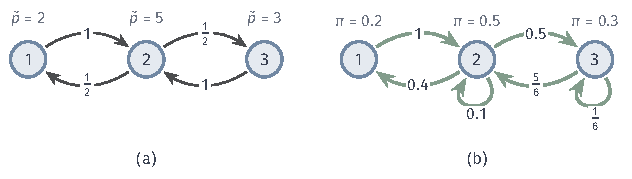
\includegraphics[width=107mm]{figures/07-probability/08-sampling-and-integration/tikz/sgen-mh-three-state/figure.pdf}
  \caption{三状态目标$\widetilde{p}=(2,5,3)$上的Metropolis--Hastings。(a)建议$q$：从端点总是走向中间，从中间各以$1/2$走向两端；(b)修正后的转移核，绿色箭头上是转移概率，自环来自拒绝。两个方向的概率流相等：$1\leftrightarrow2$都是$0.2$，$2\leftrightarrow3$都是$0.25$。}
  \label{fig:sgen-mh-three-state}
\end{BookInlineFigure}

若省去建议比，只用$\min\{1,\widetilde{p}(y)/\widetilde{p}(x)\}$，则$a(2,1)=0.4$、$a(2,3)=0.6$、$a(1,2)=a(3,2)=1$，转移矩阵的第二行变为$(0.2,0.5,0.3)$，第一、三行都是$(0,1,0)$。解$\pi\bm{K}=\pi$，由第一列得$\pi(1)=0.2\pi(2)$，由第三列得$\pi(3)=0.3\pi(2)$，归一化后
\[
  \pi=\Bigl(\frac{2}{15},\ \frac{2}{3},\ \frac{1}{5}\Bigr)\ne(0.2,\ 0.5,\ 0.3).
\]
中间状态被建议得多，又没有被修正，于是被过度访问。

\paragraph{随机游走建议}
连续状态最常用的建议是在当前点加一个对称扰动，$y=x+s\,\varepsilon$，$\varepsilon\sim\mathcal{N}(0,1)$，称为\term{随机游走Metropolis算法}（random-walk Metropolis algorithm）。步长$s$决定了接受率与移动距离之间的取舍。图~\ref{fig:sgen-rwmh-traces}在全章的混合目标上从$x=-2$出发各运行$3000$步：$s=0.3$时接受率约$0.83$，每步移动很小，链在左峰停留了很久，只有约$8\%$的时间在右边（目标是$70\%$）；$s=30$时几乎每个候选都落在目标概率很小的远处，接受率约$0.064$，链大段时间原地不动；$s=2.5$时接受率约$0.47$，两峰之间往来频繁。

\begin{BookInlineFigure}
  \centering
  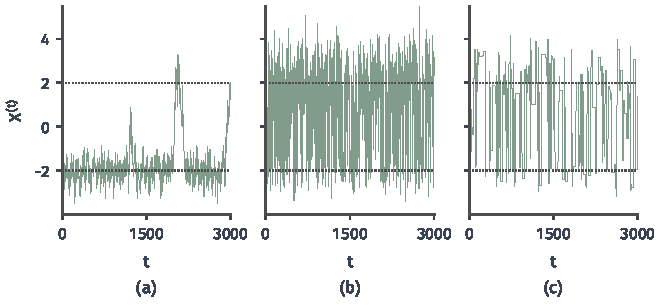
\includegraphics[width=112mm]{figures/07-probability/08-sampling-and-integration/matplotlib/sgen-rwmh-traces/figure.pdf}
  \caption{随机游走Metropolis在混合目标$0.3\,\mathcal{N}(-2,0.5^{2})+0.7\,\mathcal{N}(2,1)$上的轨迹，从$x=-2$出发，各$3000$步（种子$9$），虚线标出两个峰的位置。(a)$s=0.3$，接受率$0.83$；(b)$s=2.5$，接受率$0.47$；(c)$s=30$，接受率$0.064$，水平段是连续的拒绝。}
  \label{fig:sgen-rwmh-traces}
\end{BookInlineFigure}

三条链的转移都以同一个混合分布为不变分布，定理~\ref{thm:sgen-mh}对它们一视同仁。它们的差别全在“多快走遍目标”上，这是不变性之外的性质。每一步的成本是一次建议抽样、一次$\widetilde{p}$求值（当前点的值可以保存）和一个基础随机数。高维或尾部很重时，$\widetilde{p}$可能下溢为$0$或上溢，实际计算一律比较$\ln u_{\mathrm{a}}$与$\ln\widetilde{p}(y)-\ln\widetilde{p}(x)$加上建议比的对数。

\paragraph{建议必须能连通目标的支持}
不变性对任何建议都成立，包括那些根本到不了目标某些部分的建议。设目标是$[0,1]\cup[3,4]$上的均匀分布，建议是$y\sim\operatorname{Unif}(x-h,x+h)$。取$h=0.5$，从$x\in[0,1]$出发，候选落在$[x-0.5,x+0.5]\subset[-0.5,1.5]$中，凡是落在$[0,1]$之外的都有$\widetilde{p}(y)=0$而被拒绝，所以链永远留在$[0,1]$里。目标有一半质量在$[3,4]$上，链却一次也看不到。取$h=2.5$，候选可以越过长为$2$的空隙，链在两段之间往来（图~\ref{fig:sgen-mh-gap}）。

\begin{BookInlineFigure}
  \centering
  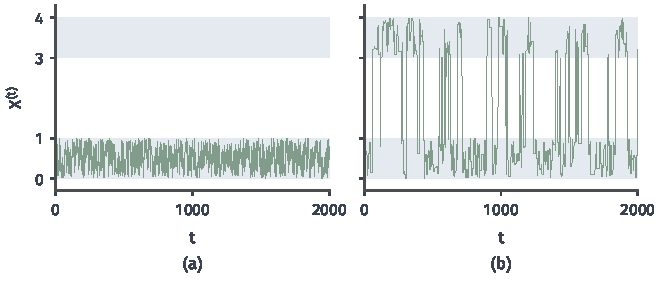
\includegraphics[width=112mm]{figures/07-probability/08-sampling-and-integration/matplotlib/sgen-mh-gap/figure.pdf}
  \caption{目标为$[0,1]\cup[3,4]$上的均匀分布（浅蓝带），建议为$\operatorname{Unif}(x-h,x+h)$，从$x=0.5$出发$2000$步（种子$10$）。(a)$h=0.5$：候选无法越过空隙，链停在$[0,1]$中，在$[3,4]$中的时间比例为$0$；(b)$h=2.5$：链在两段间往来，$[3,4]$中的时间比例为$0.39$，目标值为$0.5$。}
  \label{fig:sgen-mh-gap}
\end{BookInlineFigure}

这个例子中的失败在轨迹上一目了然，因为事先知道目标有两段。若不知道目标的形状，(a)的轨迹看起来是一条“混合良好”的链，在$[0,1]$上来回游走、接受率高达$0.75$，没有任何内部迹象提示还有一半质量没有访问。所以选择建议时，要从目标的结构出发论证它能连通支持，不能用接受公式的正确性或轨迹的外观代替这一论证。

\paragraph{独立建议}
另一种常用的建议是与当前状态无关的$q(y\mid x)=q(y)$，称为独立建议。记$w(x)=\widetilde{p}(x)/q(x)$，式~\eqref{eq:sgen-mh-acceptance}化为$\min\{1,w(y)/w(x)\}$：候选的权重比当前状态大就一定接受。它与拒绝采样用的是同一个比值，但不需要包络常数；代价是输出相关，而且若$q$在某处比目标轻得多，链一旦走到那里，$w(x)$很大，就会长时间被拒绝而停留。

\subsection{Gibbs采样}
\label{sec:sgen-gibbs}

多维目标的另一种局部信息是条件分布。设状态是$\bm{x}=(x_1,\dots,x_d)$，记$\bm{x}_{-i}$为去掉第$i$个坐标后的其余坐标。许多目标的联合分布难以直接抽样，但固定其余坐标后，第$i$个坐标的条件分布$\pi(\cdot\mid\bm{x}_{-i})$是一个熟悉的一维分布。这些条件分布称为完全条件分布。

\paragraph{单坐标更新}
保留其余坐标，只按完全条件分布重新抽第$i$个坐标，这一步的转移核记作$K_i$：从$\bm{x}$出发，新状态的第$i$个坐标服从$\pi(\cdot\mid\bm{x}_{-i})$，其余坐标与$\bm{x}$相同。轮流或随机地施行这些更新，就是\term{Gibbs采样}（Gibbs sampling）。

\begin{theorem}[单坐标更新保持目标]
\label{thm:sgen-gibbs}
设$\pi$是乘积空间上的分布，$\pi(\cdot\mid\bm{x}_{-i})$是给定其余坐标时第$i$个坐标的正则条件分布。则$\pi K_i=\pi$。
\end{theorem}

\begin{proof}
设$\bm{X}\sim\pi$，按$K_i$更新得到$\bm{X}'$，即$\bm{X}'_{-i}=\bm{X}_{-i}$，而给定$\bm{X}$时$X'_i$服从$\pi(\cdot\mid\bm{X}_{-i})$。新坐标只依赖$\bm{X}_{-i}$，旧的$X_i$在更新中被丢弃。于是$\bm{X}'_{-i}$的分布是$\pi$的边缘分布$\pi_{-i}$，给定$\bm{X}'_{-i}$时$X'_i$的条件分布是$\pi(\cdot\mid\bm{X}'_{-i})$。由第~\ref{chap:conditional-distributions}章，边缘分布与条件分布这一对确定了联合分布，它们恰好是$\pi$的边缘分布与条件分布，所以$\bm{X}'\sim\pi$。
\end{proof}

证明的直观是：更新前把$X_i$忘掉，剩下的$\bm{X}_{-i}$仍服从目标的边缘分布；再按正确的条件分布把$X_i$补回来，联合分布就复原了。也可以把单坐标更新看作建议为$q(\bm{y}\mid\bm{x})=\pi(y_i\mid\bm{x}_{-i})$的Metropolis--Hastings：此时$\bm{y}_{-i}=\bm{x}_{-i}$，比值
\[
  \frac{\pi(\bm{y})\,\pi(x_i\mid\bm{x}_{-i})}{\pi(\bm{x})\,\pi(y_i\mid\bm{x}_{-i})}=\frac{\pi_{-i}(\bm{x}_{-i})\pi(y_i\mid\bm{x}_{-i})\,\pi(x_i\mid\bm{x}_{-i})}{\pi_{-i}(\bm{x}_{-i})\pi(x_i\mid\bm{x}_{-i})\,\pi(y_i\mid\bm{x}_{-i})}=1,
\]
所以候选总被接受。

\paragraph{组合更新}
单坐标更新只动一个坐标，要让所有坐标都变化，需要把它们组合起来。按固定顺序依次施行$K_1,K_2,\dots,K_d$称为系统扫描，一轮的转移核是乘积$K_1K_2\cdots K_d$；每步以固定概率$c_i$随机选一个坐标更新，称为随机扫描，转移核是$\sum_ic_iK_i$，其中$c_i\ge0$、$\sum_ic_i=1$。两种组合都保持$\pi$：
\[
  \begin{gathered}
    \pi K_1K_2\cdots K_d=\pi K_2\cdots K_d=\dots=\pi,\\
    \pi\sum_ic_iK_i=\sum_ic_i\,\pi K_i=\sum_ic_i\pi=\pi.
  \end{gathered}
\]
随机扫描的条件是选择概率$c_i$固定，不能依赖当前状态。反例如下：设$\pi$是$\{0,1\}^{2}$上的均匀分布，规则为“$x_1=0$时更新第一个坐标，$x_1=1$时更新第二个坐标”。从$\pi$出发，$x_1=0$的一半质量更新$x_1$，其中一半变成$1$；$x_1=1$的一半质量只更新$x_2$，$x_1$保持为$1$。于是一步后
\[
  \mathbb{P}(X'_1=1)=\frac12\times\frac12+\frac12\times1=\frac34\ne\frac12 .
\]
每个$K_i$各自保持$\pi$，按状态挑选却把$x_1=1$的状态“锁住”了。

\paragraph{计算过程}
用二元高斯目标$\mathcal{N}(\bm{0},\bigl[\begin{smallmatrix}1&\rho\\\rho&1\end{smallmatrix}\bigr])$演示系统扫描，$\rho=0.8$。由第~\ref{chap:multivariate-distributions}章的高斯条件分布，两个完全条件分布是
\begin{equation}
  X_1\mid X_2=x_2\sim\mathcal{N}(\rho x_2,\,1-\rho^{2}),\qquad X_2\mid X_1=x_1\sim\mathcal{N}(\rho x_1,\,1-\rho^{2}).
  \label{eq:sgen-gibbs-gaussian}
\end{equation}

\needspace{6\baselineskip}
\paragraph{变量}
\begin{itemize}
  \item $(x_1,x_2)$：当前状态，每个坐标更新后立即覆盖。
  \item $z$：每次坐标更新使用的标准高斯数，由一个基础随机数经$\Phi^{-1}$得到。
\end{itemize}

\paragraph{初始化}
取一个初始状态。例中故意取在目标的边缘，$(x_1^{(0)},x_2^{(0)})=(2,2)$，以便看出链怎样走向中心。

\needspace{6\baselineskip}
\paragraph{每轮更新}
第$t+1$轮：
\begin{enumerate}
  \item \textbf{更新第一个坐标。}由式~\eqref{eq:sgen-gibbs-gaussian}，令
  \[
    x_1^{(t+1)}=\rho x_2^{(t)}+\sqrt{1-\rho^{2}}\,z .
  \]
  例中第一轮$z=\Phi^{-1}(0.37)\approx-0.3319$，
  \[
    x_1^{(1)}=0.8\times2+0.6\times(-0.3319)\approx1.4009 .
  \]

  \item \textbf{更新第二个坐标。}用刚得到的$x_1^{(t+1)}$，令
  \[
    x_2^{(t+1)}=\rho x_1^{(t+1)}+\sqrt{1-\rho^{2}}\,z' .
  \]
  例中第一轮$z'=\Phi^{-1}(0.80)\approx0.8416$，
  \[
    x_2^{(1)}=0.8\times1.4009+0.6\times0.8416\approx1.6257 .
  \]
  第二轮用$\Phi^{-1}(0.15)\approx-1.0364$与$\Phi^{-1}(0.62)\approx0.3055$，得到
  \[
    x_1^{(2)}\approx0.6787,\qquad x_2^{(2)}\approx0.7263 .
  \]

  \item \textbf{停止。}做满预定轮数后停止。
\end{enumerate}
最终得到状态序列$(2,2)$、$(1.4009,1.6257)$、$(0.6787,0.7263)$、\dots。每次只沿一个坐标轴移动，路径呈阶梯状。

\paragraph{相关性与移动速度}
相邻状态共用坐标，因而相关。在这个例子中可以算出相关的大小。把一轮的两步合起来，
\[
  X_1^{(t+1)}=\rho X_2^{(t)}+\sqrt{1-\rho^{2}}\,Z=\rho^{2}X_1^{(t)}+\rho\sqrt{1-\rho^{2}}\,Z''+\sqrt{1-\rho^{2}}\,Z,
\]
其中$Z''$是上一轮更新$X_2^{(t)}$所用的标准高斯数，$Z,Z''$与$X_1^{(t)}$独立。若链已处于目标分布，$\operatorname{Var}(X_1^{(t)})=1$，于是
\[
  \operatorname{Cov}\bigl(X_1^{(t+1)},X_1^{(t)}\bigr)=\rho^{2},
\]
逐轮迭代得到相隔$k$轮的相关系数为$\rho^{2k}$。$\rho=0.8$时每轮相关系数为$0.64$，几轮之后就基本忘记了起点；$\rho=0.99$时每轮为$0.98$，要约$35$轮相关系数才降到一半。

图~\ref{fig:sgen-gibbs-path}画出两种情形下前$20$轮的路径。目标沿对角线拉长时，每个完全条件分布都很窄，宽度为$\sqrt{1-\rho^{2}}$，链只能沿坐标轴迈小步，在狭长的山脊上缓慢挪动。这是Gibbs采样的典型弱点：坐标之间强相关时移动很慢，此时把强相关的坐标合成一块整体更新，或者换一套坐标，会有明显改善。

\begin{BookInlineFigure}
  \centering
  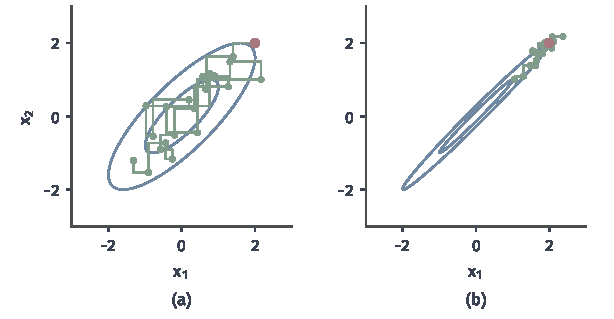
\includegraphics[width=104mm]{figures/07-probability/08-sampling-and-integration/matplotlib/sgen-gibbs-path/figure.pdf}
  \caption{二元高斯目标上的系统扫描Gibbs采样，从红点$(2,2)$出发$20$轮，前两轮使用正文中的随机数，其后的标准高斯数取自种子$12$。蓝色椭圆是目标的$1$倍与$2$倍等概率线，绿色阶梯是路径，绿点是每轮结束时的状态。(a)$\rho=0.8$，链很快进入中心并四处移动；(b)$\rho=0.99$，同样的随机数下链只沿山脊挪动了一小段。}
  \label{fig:sgen-gibbs-path}
\end{BookInlineFigure}

\paragraph{条件更新可能走不通}
Gibbs采样只沿坐标轴移动，目标的支持形状可能挡住去路。设目标是$[0,1]^{2}\cup[2,3]^{2}$上的均匀分布。当$x_2\in[0,1]$时，$x_1$的完全条件分布是$[0,1]$上的均匀分布，因为水平线$\{x_2=\text{常数}\}$只与下面的正方形相交；同理$x_1\in[0,1]$时$x_2$也只能在$[0,1]$中取值。从下面的正方形出发，链永远留在那里，尽管每一步都正确地保持了目标。若把两个正方形改成相互重叠的$[0,2]^{2}\cup[1,3]^{2}$，穿过重叠带的水平线同时碰到两个正方形，链就可以过去（图~\ref{fig:sgen-gibbs-reducible}）。

\begin{BookInlineFigure}
  \centering
  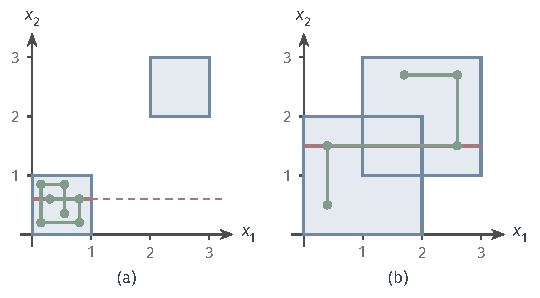
\includegraphics[width=91mm]{figures/07-probability/08-sampling-and-integration/tikz/sgen-gibbs-reducible/figure.pdf}
  \caption{支持形状对Gibbs采样的影响，目标是浅蓝区域上的均匀分布。(a)两个正方形在两个坐标方向上都不重叠，红色实线是$x_2=0.6$时$x_1$的条件分布所在区间，延长的红色虚线碰不到另一个正方形，绿色路径永远留在下方；(b)两个正方形部分重叠，红线$x_2=1.5$同时穿过两者，绿色路径经由它进入上方的正方形。}
  \label{fig:sgen-gibbs-reducible}
\end{BookInlineFigure}

每轮Gibbs采样的成本是$d$次条件抽样。完全条件分布是标准分布时，每次只需常数个基础随机数；不是标准分布时，每次条件抽样可能要用逆变换的数值反演、拒绝采样，甚至在这一坐标上做一步Metropolis--Hastings。后一种做法仍保持$\pi$，因为它是一个以$\pi(\cdot\mid\bm{x}_{-i})$为不变分布的一维更新，套上定理~\ref{thm:sgen-gibbs}的证明即可。

\subsection{Hamilton采样}
\label{sec:sgen-hmc}

随机游走建议和坐标更新都只能迈小步：步子大了接受率就低，坐标强相关时又只能沿轴挪动。若目标在欧氏空间上有光滑的正密度，梯度给出了“往哪里走概率不会掉太多”的信息。Hamilton采样借用力学中的运动方程，沿着保持总能量的轨道一次走出很远，再用接受判定修正数值误差\scite{pgm-sampling-neal2011}。

\paragraph{辅助动量与Hamilton量}
设目标为$\pi(\bm{x})\propto\exp(-U(\bm{x}))$，$\bm{x}\in\mathbb{R}^{d}$，其中$U=-\ln\widetilde{p}$二阶连续可微，称为势能。引入与$\bm{x}$同维、相互独立的辅助变量$\bm{p}\sim\mathcal{N}(\bm{0},\bm{I})$，称为动量。$(\bm{x},\bm{p})$的联合密度正比于
\begin{equation}
  \exp\bigl(-H(\bm{x},\bm{p})\bigr),\qquad H(\bm{x},\bm{p})=U(\bm{x})+\tfrac12\lVert\bm{p}\rVert_2^{2},
  \label{eq:sgen-hamiltonian}
\end{equation}
$H$称为Hamilton量，第二项是动能。联合密度分解为$\bm{x}$的因子与$\bm{p}$的因子之积，所以$\bm{x}$的边缘分布就是$\pi$：只要构造出保持联合分布的链，丢掉动量即可。

在相空间中沿Hamilton方程
\[
  \frac{\mathrm{d}\bm{x}}{\mathrm{d}t}=\bm{p},\qquad \frac{\mathrm{d}\bm{p}}{\mathrm{d}t}=-\nabla U(\bm{x})
\]
运动，有两条关键性质：$H$沿轨道守恒，相空间体积在流映射下保持不变，可参考\BookChapterRef{chap:ode-sensitivity}{卷六第4章“解的敏感性”}。$H$守恒意味着联合密度沿轨道不变，体积保持意味着把一块区域搬走时不需要Jacobian修正。轨道可以穿过目标的大片区域，同时停留在同一个密度水平上，这正是随机游走做不到的。

\paragraph{确定性提议的接受判定}
精确的Hamilton流一般解不出来，要用数值格式近似。先说明：任何满足两个条件的确定性映射，都可以配上一道接受判定而精确保持目标。

\begin{lemma}[对合映射的Metropolis修正]
\label{lem:sgen-involution}
设$\rho$是$\mathbb{R}^{m}$上的概率密度，$\Phi:\mathbb{R}^{m}\to\mathbb{R}^{m}$满足$\Phi\circ\Phi=\mathrm{id}$（对合），且保持体积（$\lvert\det D\Phi\rvert\equiv1$）。从$\bm{z}$出发，提议$\Phi(\bm{z})$，以概率$\min\{1,\rho(\Phi(\bm{z}))/\rho(\bm{z})\}$接受，否则留在$\bm{z}$。则$\rho$满足细致平衡，因而是不变分布。
\end{lemma}

\begin{proof}
从$\bm{z}$出发、被接受的移动所带的概率流密度为
\[
  m(\bm{z})=\rho(\bm{z})\min\Bigl\{1,\frac{\rho(\Phi(\bm{z}))}{\rho(\bm{z})}\Bigr\}=\min\bigl\{\rho(\bm{z}),\rho(\Phi(\bm{z}))\bigr\},
\]
$\rho(\bm{z})=0$时两边都取$0$。由$\Phi\circ\Phi=\mathrm{id}$，把$\bm{z}$换成$\Phi(\bm{z})$只是交换最小值中的两项，所以
\[
  m(\Phi(\bm{z}))=m(\bm{z}).
\]对可测集$A,B$，从$A$经接受的移动进入$B$的流量为
\[
  \int\mathbf{1}_{A}(\bm{z})\,\mathbf{1}_{B}(\Phi(\bm{z}))\,m(\bm{z})\,\mathrm{d}\bm{z}.
\]
作换元$\bm{z}=\Phi(\bm{w})$。由体积保持，体积元不变；由对合，$\Phi(\bm{z})=\bm{w}$；再由$m$在$\Phi$下不变，上式化为
\[
  \int\mathbf{1}_{A}(\Phi(\bm{w}))\,\mathbf{1}_{B}(\bm{w})\,m(\bm{w})\,\mathrm{d}\bm{w},
\]
这正是从$B$经接受的移动进入$A$的流量。被拒绝时留在原地，这部分流量对$A,B$对称。所以式~\eqref{eq:sgen-detailed-balance}成立，由引理~\ref{lem:sgen-detailed-balance}，$\rho$是不变分布。
\end{proof}

两个条件各有作用。对合使提议“可以原路返回”：从$\bm{z}$提议$\Phi(\bm{z})$，从$\Phi(\bm{z})$恰好提议回$\bm{z}$，正反两个方向成对出现。体积保持使换元时不出现Jacobian因子，接受概率只是密度之比。缺了体积保持，比值中还要乘上$\lvert\det D\Phi(\bm{z})\rvert$。

\paragraph{蛙跳格式}
求解Hamilton方程的\term{蛙跳格式}（leapfrog scheme）以步长$\varepsilon$做三个子步：
\begin{equation}
  \bm{p}_{1/2}=\bm{p}-\frac{\varepsilon}{2}\nabla U(\bm{x}),\qquad
  \bm{x}'=\bm{x}+\varepsilon\,\bm{p}_{1/2},\qquad
  \bm{p}'=\bm{p}_{1/2}-\frac{\varepsilon}{2}\nabla U(\bm{x}'),
  \label{eq:sgen-leapfrog}
\end{equation}
记这一步为$\Psi_{\varepsilon}:(\bm{x},\bm{p})\mapsto(\bm{x}',\bm{p}')$。

它保持体积：三个子步各自只改变一组变量，改变量只依赖另一组变量，例如第一步$(\bm{x},\bm{p})\mapsto(\bm{x},\bm{p}-\tfrac{\varepsilon}{2}\nabla U(\bm{x}))$的Jacobian矩阵是分块下三角的，对角块都是单位矩阵，行列式为$1$。三个这样的映射复合，行列式仍为$1$。

它在动量反转下可逆。记$F(\bm{x},\bm{p})=(\bm{x},-\bm{p})$。从$(\bm{x}',-\bm{p}')$再做一步$\Psi_{\varepsilon}$，三个子步依次给出
\[
  \begin{aligned}
    -\bm{p}'-\tfrac{\varepsilon}{2}\nabla U(\bm{x}')&=-\bm{p}_{1/2},\\
    \bm{x}'+\varepsilon(-\bm{p}_{1/2})&=\bm{x},\\
    -\bm{p}_{1/2}-\tfrac{\varepsilon}{2}\nabla U(\bm{x})&=-\bm{p},
  \end{aligned}
\]
第一行用到式~\eqref{eq:sgen-leapfrog}的第三式，第二、三行用到第二式和第一式。所以先走一步、反转、再走一步，得到的是$(\bm{x},-\bm{p})$，即$\Psi_{\varepsilon}F\Psi_{\varepsilon}=F$。由$F\circ F=\mathrm{id}$，这等价于$F\Psi_{\varepsilon}F=\Psi_{\varepsilon}^{-1}$。连做$L$步时，
\[
  F\Psi_{\varepsilon}^{L}F=(F\Psi_{\varepsilon}F)^{L}=\Psi_{\varepsilon}^{-L},
\]
所以$\Phi=F\circ\Psi_{\varepsilon}^{L}$满足$\Phi\circ\Phi=\mathrm{id}$，并且保持体积。精确的Hamilton流有同样两条性质，蛙跳格式在离散后仍完整保留了它们，失去的只是$H$的守恒。

\paragraph{完整的一步}
\term{Hamilton采样}（Hamiltonian Monte Carlo）的一步由两部分组成：
\begin{enumerate}
  \item \textbf{刷新动量。}丢弃旧的动量，重新抽$\bm{p}\sim\mathcal{N}(\bm{0},\bm{I})$。在联合分布下$\bm{p}$与$\bm{x}$独立，这一步就是对$\bm{p}$的一次Gibbs更新，由定理~\ref{thm:sgen-gibbs}，它保持联合分布。

  \item \textbf{轨道提议与修正。}从$(\bm{x},\bm{p})$出发做$L$步蛙跳，再反转动量，得到
  \[
    (\bm{x}^{*},\bm{p}^{*})=F\Psi_{\varepsilon}^{L}(\bm{x},\bm{p}),
  \]
  以概率
  \begin{equation}
    \min\Bigl\{1,\ \exp\bigl(H(\bm{x},\bm{p})-H(\bm{x}^{*},\bm{p}^{*})\bigr)\Bigr\}
    \label{eq:sgen-hmc-accept}
  \end{equation}
  接受$\bm{x}^{*}$，否则保留$\bm{x}$。由引理~\ref{lem:sgen-involution}（取$\rho\propto\mathrm{e}^{-H}$），这一步也保持联合分布。
\end{enumerate}
两步复合仍保持联合分布，于是$\bm{x}$的边缘分布$\pi$不变。式~\eqref{eq:sgen-hmc-accept}只用到$U$的值差，归一化常数照样约掉。

四个组成部分各司其职。刷新动量改变能量水平：若不刷新，链只在一条近似的能量等值面上移动，无法到达其他密度水平。蛙跳格式的可逆与保体积使接受概率只含能量差。动量反转把提议变成对合，满足引理的条件；下一步开始时动量会被重新抽取，而$\mathcal{N}(\bm{0},\bm{I})$关于$\bm{p}\mapsto-\bm{p}$对称，所以实际程序中常省去这一反转。接受判定修正离散化误差：精确流下$H$守恒，接受概率为$1$，蛙跳的能量误差越小，接受率越高。

\paragraph{计算过程}
用一维标准高斯目标演示，$U(x)=x^{2}/2$，$\nabla U(x)=x$，步长$\varepsilon=0.5$，每次提议走$L=2$步。

\needspace{6\baselineskip}
\paragraph{变量}
\begin{itemize}
  \item $x$：当前位置；$p$：本次刷新的动量。
  \item $(x_{\ell},p_{\ell})$：蛙跳第$\ell$步后的位置与动量，$\ell=0,\dots,L$。
  \item $\Delta H$：轨道终点与起点的能量差。
\end{itemize}

\paragraph{初始化}
给定当前位置。例中$x=1$。

\needspace{6\baselineskip}
\paragraph{每轮更新}
\begin{enumerate}
  \item \textbf{刷新动量。}抽$p\sim\mathcal{N}(0,1)$。例中由$u=0.80$得$p=\Phi^{-1}(0.80)\approx0.8416$，于是
  \[
    H(x_0,p_0)=\frac{1^{2}}{2}+\frac{0.8416^{2}}{2}\approx0.8542 .
  \]

  \item \textbf{蛙跳$L$步。}按式~\eqref{eq:sgen-leapfrog}迭代。例中第一步
  \[
    \begin{aligned}
      p_{1/2}&=0.8416-0.25\times1=0.5916,\\
      x_1&=1+0.5\times0.5916=1.2958,\\
      p_1&=0.5916-0.25\times1.2958\approx0.2677 .
    \end{aligned}
  \]
  第二步
  \[
    \begin{aligned}
      p_{3/2}&\approx0.2677-0.25\times1.2958=-0.0563,\\
      x_2&\approx1.2958+0.5\times(-0.0563)=1.2677,\\
      p_2&\approx-0.0563-0.25\times1.2677=-0.3732 .
    \end{aligned}
  \]

  \item \textbf{反转并计算能量差。}令$p^{*}=-p_2$，它不改变动能。例中
  \[
    H(x_2,p^{*})=\frac{1.2677^{2}}{2}+\frac{0.3732^{2}}{2}\approx0.8731,\qquad \Delta H\approx0.0190 .
  \]

  \item \textbf{判定。}由式~\eqref{eq:sgen-hmc-accept}，接受概率为$\min\{1,\mathrm{e}^{-\Delta H}\}$。例中$\mathrm{e}^{-0.0190}\approx0.9812$，取基础随机数$u=0.37$，接受，新位置为$1.2677$。
\end{enumerate}
最终一次迭代用到$x_0,x_1,x_2$三处的梯度（$x_1$处的梯度在两步之间重复使用）和两个基础随机数，位置从$1$移到$1.2677$。能量只变了约$0.019$，所以几乎必然接受。

\paragraph{步长与轨道长度}
步长决定能量误差。对这个一维例子，式~\eqref{eq:sgen-leapfrog}是线性映射，代入$\nabla U(x)=x$可得
\[
  \begin{bmatrix}x'\\p'\end{bmatrix}=
  \begin{bmatrix}1-\varepsilon^{2}/2&\varepsilon\\-\varepsilon(1-\varepsilon^{2}/4)&1-\varepsilon^{2}/2\end{bmatrix}
  \begin{bmatrix}x\\p\end{bmatrix}.
\]
矩阵的行列式为$1$，迹为$2-\varepsilon^{2}$。$0<\varepsilon<2$时迹的绝对值小于$2$，两个特征值是单位圆上的一对共轭复数，迭代点在一个椭圆上转动，能量误差有界；$\varepsilon>2$时有一个特征值的绝对值大于$1$，轨道按指数发散，接受率趋于零。若目标的标准差为$\sigma$，同样的计算给出稳定条件$\varepsilon<2\sigma$；多维时由最窄的方向决定。

图~\ref{fig:sgen-leapfrog}(a)画出$\varepsilon=0.5$与$\varepsilon=1.8$的轨道，前者紧贴精确的圆形轨道，后者被拉成扁椭圆。(b)是固定轨道总长约为$3$时，轨道上最大能量误差随$\varepsilon$的变化，在稳定范围内大致与$\varepsilon^{2}$成正比。对一般的光滑$U$，固定轨道长度时能量误差为$O(\varepsilon^{2})$，证明要用到数值积分的误差分析，这里只用图中的数值说明。

\begin{BookInlineFigure}
  \centering
  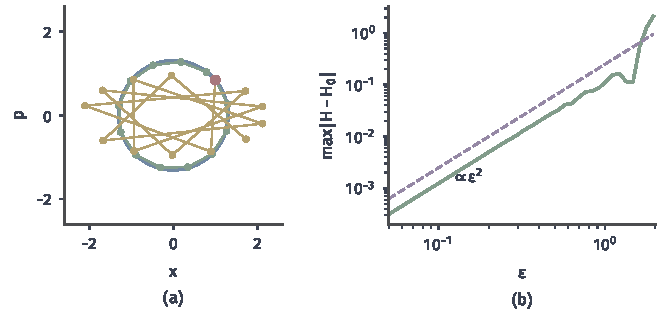
\includegraphics[width=112mm]{figures/07-probability/08-sampling-and-integration/matplotlib/sgen-leapfrog/figure.pdf}
  \caption{标准高斯目标的蛙跳格式，起点为红点$(x,p)=(1,\Phi^{-1}(0.8))$。(a)蓝线是精确的Hamilton轨道（能量等值线），绿色是$\varepsilon=0.5$的$12$步，黄色是$\varepsilon=1.8$的$12$步；(b)轨道总长约为$3$（$L=\operatorname{round}(3/\varepsilon)$）时轨道上的最大能量误差，紫色虚线是斜率为$2$的参考线。}
  \label{fig:sgen-leapfrog}
\end{BookInlineFigure}

轨道长度$L\varepsilon$决定一次能走多远。太短时与随机游走无异；太长时轨道可能绕回起点附近，例如标准高斯的精确轨道周期为$2\pi$，走满一周等于白走。每次提议的成本是$L$次梯度计算，比较方法时应在相同的梯度或密度计算次数下比较。图~\ref{fig:sgen-hmc-rw}在相关系数为$0.95$的二元高斯目标上做了这样的比较：$200$次密度计算的随机游走Metropolis（接受率$0.69$）还在山脊的一端徘徊，$200$次梯度计算的Hamilton采样（$20$次提议，每次$10$步，接受率$0.85$）已在整个椭圆上来回。

\begin{BookInlineFigure}
  \centering
  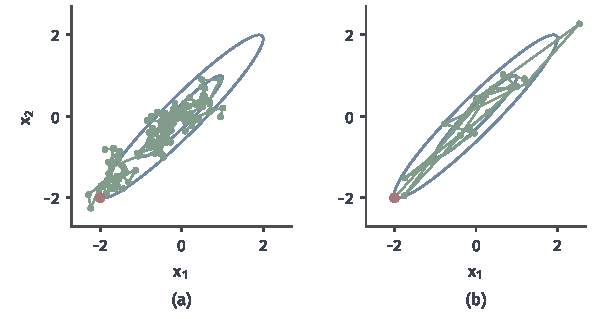
\includegraphics[width=104mm]{figures/07-probability/08-sampling-and-integration/matplotlib/sgen-hmc-rw/figure.pdf}
  \caption{相关系数$0.95$的二元高斯目标，从红点$(-2,-2)$出发，计算量相同。(a)随机游走Metropolis，步长$0.25$，$200$步；(b)Hamilton采样，$\varepsilon=0.18$、$L=10$，$20$次提议。两者都用种子$13$，蓝色椭圆是$1$倍与$2$倍等概率线。}
  \label{fig:sgen-hmc-rw}
\end{BookInlineFigure}

Hamilton采样的适用范围也由它的条件划定。它需要欧氏空间上光滑、处处为正的密度和可以计算的梯度，离散变量或有硬边界的支持都要另行处理。多峰目标中，两个峰之间的低密度区要靠刷新动量时偶尔得到的高能量才能越过，峰间隔得远时同样会长期困在一个峰中。
